\section{积分泛函}
\label{sec:func-integral}

前几节的目标$E$和$\ell$都是沿区间累加一个局部代价。于是要问：对这一类目标，最优性条件具体是什么？答案是一个常微分方程，加上由约束决定的边界条件。

设$F(x,s,p)$是定义在$[a,b]\times\mathbb{R}\times\mathbb{R}$上的函数，称为\term{密度}（density），对$(s,p)$连续可微，偏导数连续。\term{积分泛函}（integral functional）是
\begin{equation}
 J(u)=\int_a^bF\bigl(x,u(x),u'(x)\bigr)\,\mathrm{d}x.
 \label{eq:func-integral}
\end{equation}
下面用$F_s,F_p$表示$F$对第二、第三个变量的偏导数，沿候选求值时省略自变量，即$F_p$表示$F_p(x,u(x),u'(x))$，它是$x$的函数。$F_p$是对“斜率所在的变量”求偏导，不是对函数$u'$求导。

\paragraph{一阶变分}
沿直线$u+t\eta$求导，只需把导数换到积分号内。

\begin{theorem}[积分泛函的一阶变分]
\label{thm:func-first-variation}
设$u,\eta\in C^1[a,b]$。则
\begin{equation}
 J'(u;\eta)=\int_a^b\bigl(F_s\,\eta+F_p\,\eta'\bigr)\,\mathrm{d}x.
 \label{eq:func-first-variation}
\end{equation}
\end{theorem}

\begin{proof}
函数$(x,t)\mapsto F(x,u+t\eta,u'+t\eta')$对$t$的偏导数是$F_s\eta+F_p\eta'$在点$(x,u+t\eta,u'+t\eta')$的值，它在紧集$[a,b]\times[-1,1]$上连续。连续偏导数允许在积分号下求导，令$t=0$即得。
\end{proof}

这也是方向导数的线性公式。$J'(u;\eta)$对$\eta$线性，并被$\eta$的$C^1$范数控制。对Sobolev函数，要在积分号下求导还需要控制收敛定理所要求的可积上界，要根据$F$的增长条件逐项核对；$E$和$\ell$的情形已由第~\ref{sec:func-directional}节的展开直接得到。

\subsection{Euler--Lagrange方程}
\label{sec:func-euler-lagrange}

\paragraph{用分部积分消去$\eta'$}
一阶变分同时含$\eta$和$\eta'$，而它们不是独立的。为了让式子只含$\eta$，把$\eta'$前的系数移走。设$u\in C^2[a,b]$，$F$二阶连续可微，分部积分得到
\begin{equation}
 J'(u;\eta)=\int_a^b\Bigl(F_s-\frac{\mathrm{d}}{\mathrm{d}x}F_p\Bigr)\eta\,\mathrm{d}x+\Bigl[F_p\,\eta\Bigr]_a^b.
 \label{eq:func-first-variation-parts}
\end{equation}
边界项先记下来。固定端点时，可行扰动在两端为零，边界项消失。第~\ref{sec:func-free-boundary}小节放开端点时，这一项会成为主角。

此时括号里的函数在$L^2$内积下正是$J$的梯度。由第~\ref{sec:func-hilbert-gradient}小节，$E$在$u=x$处的$L^2$梯度是$x$，这里$-u''+u=x$，两者一致。驻定条件要求这个梯度与所有扰动正交，接下来把“正交于所有扰动”变成“等于零”。

\paragraph{变分基本引理}
在有限维中，若$\bm{g}^\top\bm{d}=0$对每个$\bm{d}$成立，取$\bm{d}=\bm{g}$得$\bm{g}=\bm{0}$。函数空间里扰动有端点和光滑性要求，不能直接取$\eta=g$，但可以取一个局部的小凸起，见图~\ref{fig:func-bump-lemma}。

\begin{lemma}[变分基本引理]
\label{lem:func-fundamental}
设$g\in C[a,b]$，且对每个在$(a,b)$内紧支撑的光滑函数$\eta$都有$\int_a^bg\,\eta\,\mathrm{d}x=0$。则$g\equiv0$。
\end{lemma}

\begin{proof}
设有$x_0\in(a,b)$使$g(x_0)>0$，$g(x_0)<0$的情形相同。由连续性，存在$r>0$，使$(x_0-r,x_0+r)\subset(a,b)$，且$g$在其上为正。取$\eta$为支撑在这个区间内的非负光滑函数，例如当$\lvert x-x_0\rvert<r$时
\[
 \eta(x)=\exp\Bigl(\frac{-1}{1-(x-x_0)^2/r^2}\Bigr),
\]
其余位置为零。则$g\eta\geq0$，在$x_0$处严格为正，于是积分为正，与假设矛盾。所以$g$在$(a,b)$内为零，由连续性在端点也为零。
\end{proof}

\begin{BookInlineFigure}
  \centering
  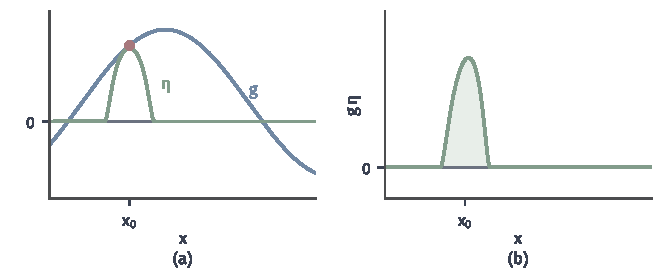
\includegraphics[width=112mm]{figures/05-optimization/08-functional-optimization/matplotlib/func-bump-lemma/figure.pdf}
  \caption{变分基本引理的构造。(a)蓝色$g$在红点$x_0$处为正，绿色凸起$\eta$只在$g>0$的小区间内非零。(b)乘积$g\eta$非负，积分严格为正，所以$g$不能与所有扰动正交。}
  \label{fig:func-bump-lemma}
\end{BookInlineFigure}

把扰动限制在局部，等于“单独改动一小段曲线”。这是向量情形“单独改动一个坐标”的连续版本：极小点处每一小段都不能再改进，方程因此对每个$x$成立。

\begin{theorem}[Euler--Lagrange方程]
\label{thm:func-euler-lagrange}
设$F$二阶连续可微，$u\in C^2[a,b]$满足$u(a)=\alpha$，$u(b)=\beta$，并且在固定端点的$C^1$函数中，是$C^1$范数下$J$的局部极小点。则对每个$x\in[a,b]$，
\begin{equation}
 \frac{\mathrm{d}}{\mathrm{d}x}F_p\bigl(x,u(x),u'(x)\bigr)=F_s\bigl(x,u(x),u'(x)\bigr).
 \label{eq:func-euler-lagrange}
\end{equation}
\end{theorem}

\begin{proof}
可行方向是端点为零的$C^1$函数，它们组成子空间，由定理~\ref{thm:func-first-order}得$J'(u;\eta)=0$。式~\eqref{eq:func-first-variation-parts}的边界项为零，再由引理~\ref{lem:func-fundamental}，括号内的连续函数恒为零。
\end{proof}

式~\eqref{eq:func-euler-lagrange}称为\term{Euler--Lagrange方程}（Euler--Lagrange equation），它的解称为\term{极值曲线}（extremal）。这个名称有些误导，因为解不一定是极值，下面专门讨论这一点。

\paragraph{两个例子}
对长度目标~\eqref{eq:func-length}，$F=\sqrt{1+p^2}$不依赖$s$，所以$F_s=0$，方程~\eqref{eq:func-euler-lagrange}说$F_p$是常数：
\[
 \frac{u'(x)}{\sqrt{1+u'(x)^2}}=c.
\]
函数$p\mapsto p/\sqrt{1+p^2}$严格递增，所以$u'$是常数，$u$是直线。加上端点条件得$u(x)=x$，$\ell^\star=\sqrt2$。

对能量~\eqref{eq:func-energy}，$F=\frac12p^2+\frac12s^2$，$F_p=p$，$F_s=s$，方程是
\begin{equation}
 u''=u,\qquad u(0)=0,\ u(1)=1.
 \label{eq:func-energy-el}
\end{equation}
通解是$A\sinh x+B\cosh x$，由$u(0)=0$得$B=0$，由$u(1)=1$得$A=1/\sinh1$，于是
\begin{equation}
 u^\star(x)=\frac{\sinh x}{\sinh1}.
 \label{eq:func-energy-solution}
\end{equation}
这就是第~\ref{sec:func-hilbert-gradient}小节由一步梯度得到的曲线。由$u''=u$，有$u'^2+u^2=(uu')'$，积分得到最优值
\begin{equation}
 E^\star=\frac12\bigl[uu'\bigr]_0^1=\frac12u'(1)=\frac12\coth1\approx0.6565.
 \label{eq:func-energy-value}
\end{equation}
$E$严格凸，由定理~\ref{thm:func-convex-sufficient}，$u^\star$就是唯一的全局最优解。

\paragraph{函数要有多光滑}
推导用了$u\in C^2$，它只是为了分部积分。候选只有$C^1$时，换一个方向分部积分，把导数放到$F_s$的原函数上。令$A(x)=\int_a^xF_s\,\mathrm{d}\tau$，它是$C^1$函数。分部积分，由$\eta$在端点为零得到
\[
 \int_a^bF_s\eta\,\mathrm{d}x=-\int_a^bA\eta'\,\mathrm{d}x.
\]
于是驻定条件变成
\[
 \int_a^b(F_p-A)\,\eta'\,\mathrm{d}x=0\qquad\text{对端点为零的}\ \eta\in C^1.
\]

下面的引理把这个条件化成$F_p-A$是常数。设$g\in C[a,b]$满足$\int_a^bg\eta'\,\mathrm{d}x=0$。令$c$为$g$的平均值，取$\eta(x)=\int_a^x(g-c)\,\mathrm{d}\tau$，它在两端为零，由$\int_a^b\eta'\,\mathrm{d}x=0$得到
\[
 \int_a^b(g-c)^2\,\mathrm{d}x=\int_a^b(g-c)\eta'\,\mathrm{d}x=\int_a^bg\eta'\,\mathrm{d}x=0.
\]
所以$g\equiv c$。这一结论称为du Bois-Reymond引理。把它用在$g=F_p-A$上，得到积分形式的方程
\begin{equation}
 F_p\bigl(x,u(x),u'(x)\bigr)=c+\int_a^xF_s\,\mathrm{d}\tau.
 \label{eq:func-du-bois}
\end{equation}
右端是$C^1$的，所以$F_p$沿曲线可导且满足式~\eqref{eq:func-euler-lagrange}，虽然$u''$可能不存在。若$F_{pp}>0$，由隐函数定理可从$F_p$解出$u'$，$u$自动属于$C^2$。

式~\eqref{eq:func-du-bois}对分段$C^1$的候选同样成立，而右端连续，所以在曲线的折点处，$F_p$不能跳变。这是极值曲线可以有折点的唯一条件。对$G(p)=(p^2-1)^2$，$F_p=4p(p^2-1)$在$p=\pm1$处都为零，所以斜率$\pm1$的锯齿满足这个条件。而钉子问题中$F_p=u'$在中点跳变，因为那里的扰动受到约束，驻定条件只对$\eta(\frac12)=0$的方向成立，跳变的幅度$4$正是乘子。

对$H^1$中的极小点，能直接得到的只有弱形式：$\int_a^b(F_s\eta+F_p\eta')\,\mathrm{d}x=0$。极小点是否足够光滑从而满足方程的经典形式，是方程理论的正则性问题，可参考\BookChapterRef{chap:elliptic-equations}{卷六第7章“椭圆方程”}。

\paragraph{方程是必要条件}
式~\eqref{eq:func-euler-lagrange}由“若是局部极小点”推出，反过来不成立。对目标~\eqref{eq:func-rho}，$F_p=p$，$F_s=-\rho s$，方程是$u''+\rho u=0$，$u=0$总是解。而第~\ref{sec:func-optimality}节已经算出，$\rho>\pi^2$时$u=0$是鞍点，目标甚至无下界。

要断定一个解是极小点，有两条路。若$F$对$(s,p)$联合凸，则$J$是凸泛函，由定理~\ref{thm:func-convex-sufficient}，满足端点条件和方程的$u$就是全局最优解，这是$E$和$\ell$的情形。没有凸性时，要检查二阶变分，它的积分形式是
\begin{equation}
 \delta^2J(u;\eta)=\int_a^b\bigl(F_{ss}\,\eta^2+2F_{sp}\,\eta\eta'+F_{pp}\,\eta'^2\bigr)\,\mathrm{d}x.
 \label{eq:func-second-variation-integral}
\end{equation}

\paragraph{二阶必要条件的局部形式}
式~\eqref{eq:func-second-variation-integral}中哪一项决定符号？取一个窄的帐篷形扰动，半宽和高度都是$\varepsilon$，斜率为$\pm1$。$\eta^2$项的量级是$\varepsilon^3$，$\eta\eta'$项是$\varepsilon^2$，$\eta'^2$项是$\varepsilon$。$\varepsilon$很小时，$F_{pp}$的项占主导，高频扰动只看得见$F_{pp}$。

\begin{theorem}[Legendre条件]
\label{thm:func-legendre}
设$F$二阶连续可微，$u\in C^1[a,b]$是固定端点问题在$C^1$范数下的局部极小点。则对每个$x\in[a,b]$，
\begin{equation}
 F_{pp}\bigl(x,u(x),u'(x)\bigr)\geq0.
 \label{eq:func-legendre}
\end{equation}
\end{theorem}

\begin{proof}
设在内点$x_0$处$F_{pp}<0$，端点的情形由连续性归结到内点。由连续性，存在$c>0$和$\varepsilon_0>0$，使$\lvert x-x_0\rvert\leq\varepsilon_0$时$F_{pp}\leq-c$。对$\varepsilon<\varepsilon_0$取上述帐篷形扰动，把折点磨圆使之成为$C^1$函数，磨圆可以使下列估计的改变任意小。由式~\eqref{eq:func-second-variation-integral}，存在只依赖$F$和$u$的常数$M$，使
\[
 \delta^2J(u;\eta)\leq-2c\,\varepsilon+M\varepsilon^2.
\]
$\varepsilon$足够小时右端为负，与二阶必要条件矛盾。
\end{proof}

对目标~\eqref{eq:func-bolza}，$G''(0)=-4<0$，所以$u=0$不是局部极小点，这与第~\ref{sec:func-existence}节的观察一致：$G$在$0$附近非凸，锯齿能把目标压低。Legendre条件仍只是必要的。目标~\eqref{eq:func-local-example}在$u=0$处$F_{pp}=2>0$，$u=0$在$C^1$范数下也确实是局部极小点，但在上确界范数下不是。

\paragraph{向量值函数与多元区域}
方程可以逐分量推广。若未知量是向量值函数$\bm{u}:[a,b]\to\mathbb{R}^r$，密度为$F(x,\bm{s},\bm{p})$，每次只扰动一个分量，重复上面的论证，得到方程组
\begin{equation}
 \frac{\mathrm{d}}{\mathrm{d}x}\nabla_{\bm{p}}F=\nabla_{\bm{s}}F.
 \label{eq:func-euler-lagrange-vector}
\end{equation}
若未知量是区域$\Omega\subset\mathbb{R}^d$上的函数，目标是
\[
 J(u)=\int_\Omega F(\bm{x},u,\nabla u)\,\mathrm{d}\bm{x},
\]
分部积分换成散度定理，方程变为
\begin{equation}
 \operatorname{div}\bigl(\nabla_{\bm{p}}F\bigr)=F_s.
 \label{eq:func-euler-lagrange-div}
\end{equation}
例如$F=\frac12\lVert\bm{p}\rVert_2^2-g(\bm{x})s$给出$-\Delta u=g$。这些方程的解的理论不属于本章。

\subsection{自由边界条件}
\label{sec:func-free-boundary}

至此端点都是固定的。若端点可以移动，可行扰动就变多了，最优解要多满足一些条件。本小节要回答的问题是：多出来的扰动告诉我们什么？关键是重新核对式~\eqref{eq:func-first-variation-parts}中的边界项。

\paragraph{放开一个端点的值}
把例子改成：保留$u(1)=1$，$u(0)$不作约束。候选在$\bm{C}=\{u\in H^1(0,1):u(1)=1\}$中，扰动只需$\eta(1)=0$。设$u\in C^2$是极小点，推理分两步。

第一步，固定端点的扰动仍然允许。取两端为零的$\eta$，同样得到内部方程~\eqref{eq:func-euler-lagrange}，$u$仍满足它。第二步，把这个结论代回式~\eqref{eq:func-first-variation-parts}，积分项消失，只剩边界项。由$\eta(1)=0$，
\[
 0=J'(u;\eta)=\bigl[F_p\eta\bigr]_0^1=-F_p\bigl(0,u(0),u'(0)\bigr)\,\eta(0).
\]
$\eta(0)$可以取任意值，所以
\begin{equation}
 F_p\bigl(0,u(0),u'(0)\bigr)=0.
 \label{eq:func-natural}
\end{equation}

这样的条件称为\term{自然边界条件}（natural boundary condition），它不是提问时写下的，而是由优化自己产生的。若继续沿用固定端点的公式，方程少一个边界条件，解就不确定。第二步的逻辑也不能颠倒：必须先用内部扰动消去积分项，边界项才能单独出现。

对$E$，$F_p=u'$，条件是$u'(0)=0$。方程$u''=u$加上$u'(0)=0$，$u(1)=1$，解得
\begin{equation}
 u^\star(x)=\frac{\cosh x}{\cosh1}.
 \label{eq:func-free-solution}
\end{equation}
同样用$u'^2+u^2=(uu')'$积分，边界项中$u'(0)=0$，得到最优值
\[
 E^\star=\frac12u(1)u'(1)=\frac12\tanh1\approx0.3808.
\]
它比固定端点的$0.6565$小，因为可行集变大了。图~\ref{fig:func-natural-beta}(a)的绿线就是这个解，它在$x=0$处水平。

\paragraph{边界代价}
固定端点和自由端点是一族问题的两个极端。在左端加上代价$\frac\beta2u(0)^2$，$\beta\geq0$，目标为
\begin{equation}
 J_\beta(u)=E(u)+\frac{\beta}{2}u(0)^2,\qquad u(1)=1.
 \label{eq:func-robin}
\end{equation}
边界代价的微分是$\beta u(0)\eta(0)$，它和边界项$-F_p\eta(0)$相加，给出
\begin{equation}
 F_p\bigl(0,u(0),u'(0)\bigr)=\beta\,u(0).
 \label{eq:func-robin-condition}
\end{equation}
对$E$，这就是$u'(0)=\beta u(0)$。解$u''=u$，得到
\[
 u_\beta(x)=\frac{\cosh x+\beta\sinh x}{\cosh1+\beta\sinh1}.
\]
积分后，边界代价正好抵消左端的边界项，最优值为
\[
 J_\beta^\star=\frac12u_\beta'(1)=\frac12\cdot\frac{\sinh1+\beta\cosh1}{\cosh1+\beta\sinh1}.
\]

$\beta=0$回到自然边界，$J_0^\star=\frac12\tanh1$；$\beta\to\infty$时$u_\beta(0)\to0$，回到固定端点，$J_\beta^\star\to\frac12\coth1$。图~\ref{fig:func-natural-beta}显示了这一过渡。固定端点相当于“价格无穷大”的边界代价。

\begin{BookInlineFigure}
  \centering
  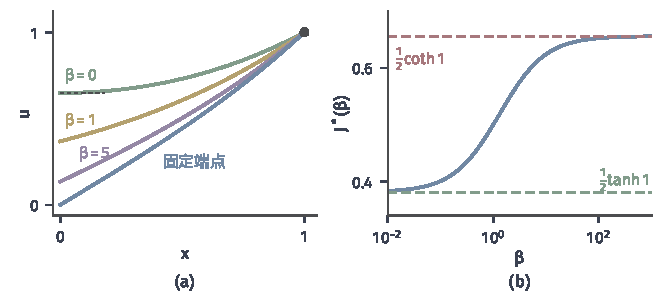
\includegraphics[width=112mm]{figures/05-optimization/08-functional-optimization/matplotlib/func-natural-beta/figure.pdf}
  \caption{从自然边界到固定端点。(a)$u(1)=1$（灰点）时，$\beta=0,1,5$的解和固定端点$u(0)=0$的解（蓝）；绿线在$x=0$处水平，短虚线是水平切线。(b)最优值$J_\beta^\star$随$\beta$从$\frac12\tanh1$上升到$\frac12\coth1$。}
  \label{fig:func-natural-beta}
\end{BookInlineFigure}

\paragraph{端点沿曲线移动}
更一般地，端点的横坐标也可以动。设左端固定在$(a,\alpha)$，右端点要落在给定曲线$y=\psi(x)$上，未知量是函数$u$和右端横坐标$b$。这时积分上限也在变，式~\eqref{eq:func-first-variation-parts}要重新推导。

取一族可行的$(u_t,b_t)$，$t=0$时为$(u,b)$，记$\eta=\partial_tu_t|_{t=0}$，$\tau=\dot{b}_t|_{t=0}$。这里$u$在$b$的右侧邻域内也有定义，$u_t$在其上可导。对积分上限和被积函数分别求导，得到
\[
 \frac{\mathrm{d}}{\mathrm{d}t}J\Big|_{t=0}=F\bigl(b,u(b),u'(b)\bigr)\tau+\int_a^b\bigl(F_s\eta+F_p\eta'\bigr)\,\mathrm{d}x.
\]
约束$u_t(b_t)=\psi(b_t)$对$t$求导，把端点的两种移动联系起来：
\[
 \eta(b)+u'(b)\tau=\psi'(b)\tau.
\]

内部方程仍然成立，因为固定$b$和端点值的扰动仍然允许。代入分部积分，并用$\eta(a)=0$，积分项消失，只剩$F\tau+F_p\eta(b)$。把上式解出的$\eta(b)=(\psi'(b)-u'(b))\tau$代入，由$\tau$可以任意取，得到
\begin{equation}
 F+\bigl(\psi'-u'\bigr)F_p=0\qquad\text{在}\ x=b.
 \label{eq:func-transversality}
\end{equation}
这是\term{横截条件}（transversality condition）。它有别于式~\eqref{eq:func-natural}，因为这里多了由积分上限移动产生的$F\tau$。

用最短曲线检验。对$F=\sqrt{1+p^2}$，式~\eqref{eq:func-transversality}化简为
\[
 \frac{1+\psi'(b)\,u'(b)}{\sqrt{1+u'(b)^2}}=0,
\]
即$\psi'(b)\,u'(b)=-1$。极值曲线是直线，所以结论是：从一点到一条曲线的最短线段垂直于这条曲线。图~\ref{fig:func-transversal}中，曲线是$\psi(x)=2-x$，斜率$-1$，于是$u'=1$。从原点出发的直线$y=x$在$(1,1)$处与之相交，长度$\sqrt2$。

\begin{BookInlineFigure}
  \centering
  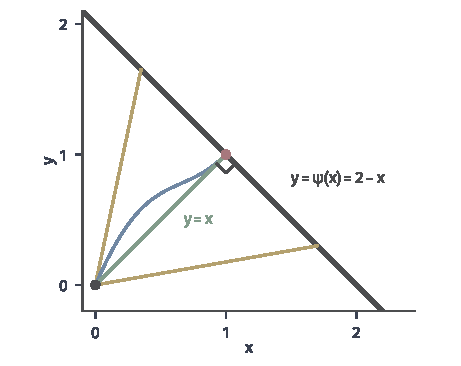
\includegraphics[width=78mm]{figures/05-optimization/08-functional-optimization/matplotlib/func-transversal/figure.pdf}
  \caption{端点沿曲线移动时的最短曲线。深灰粗线是端点可落的直线$y=2-x$，绿色线段是解，在红点$(1,1)$处与之垂直，长度$\sqrt2\approx1.414$。黄色线段端点分别在$x=0.35$和$x=1.7$处，长度分别约为$1.69$和$1.73$；蓝色曲线到同一终点，也比直线长。}
  \label{fig:func-transversal}
\end{BookInlineFigure}

\paragraph{多元区域的边界}
在区域$\Omega$上，分部积分换成散度定理，边界项变成边界积分$\int_{\partial\Omega}(\nabla_{\bm{p}}F\cdot\bm{n})\,\eta\,\mathrm{d}S$，$\bm{n}$是外法向量。边界分成两部分时，固定值的部分上$\eta=0$，放开的部分上，同样的两步推理给出$\nabla_{\bm{p}}F\cdot\bm{n}=0$。对$F=\frac12\lVert\bm{p}\rVert_2^2$，这就是法向导数为零。

各种边界情形可以总结成一张表，共同的来源都是式~\eqref{eq:func-first-variation-parts}的边界项。

\begin{BookInlineTable}
  \centering
  \caption{一维问题右端的三种边界情形，左端符号相反。}
  \label{tab:func-boundary}
  \begin{tabular}{lll}
    \toprule
    端点情形 & 允许的扰动 & 边界条件\\
    \midrule
    固定 $u(b)=\beta$ & $\eta(b)=0$ & $u(b)=\beta$\\
    放开 $u(b)$ & $\eta(b)$ 任意 & $F_p=0$\\
    放开并加代价 $\Phi(u(b))$ & $\eta(b)$ 任意 & $F_p+\Phi'(u(b))=0$\\
    沿曲线 $y=\psi(x)$ 移动 & $\eta(b)=(\psi'-u')\tau$ & $F+(\psi'-u')F_p=0$\\
    \bottomrule
  \end{tabular}
\end{BookInlineTable}
